%! Author = tstreule

\section{Ultrasound Imaging \textnormal{\normalsize $c\ped{sound} \simeq \unitfrac[1540]{m}{s}$}}

Frequencies of 1-50 MHz $\implies$ $\lambda = 1 .... 0.03 \unit{mm}$

Wave formula: $\nabla^2 p - \frac{1}{c^2} \frac{\partial^2 p}{\partial t^2} = 0$ \quad Max. p = compressional pressure= $p_c$, \quad Min. p = rarefactional pressure = $p_r$

$\kappa$ = compressibility, $\rho$ = density, $u_z$ = particle velocity\\
$c = \frac{1}{\sqrt{\kappa \rho}}$, \quad $p = \rho c u_z$, \quad $Z = p/u_z = \rho c = \sqrt{\frac{\rho}{\kappa}}$, \quad $I = p u_z / 2$

Pressure \textbf{coeff.}: \highlight{$\displaystyle r = \frac{Z_2 - Z_1}{Z_2 + Z_1}$} \highlight{$\displaystyle t = \frac{2Z_2}{Z_2 + Z_1}$}\\
\textbf{Refraction:} $\theta_i = \theta_r$, \quad $\sin\theta_i/\sin\theta_t = c_i/c_t$

\textbf{Rayleigh scattering} by structures smaller $\lambda$ $\to$ speckles/noise ($\sigma_S \propto \lambda^{-4}$). It has a char. length of $\lambda/2$:

\textbf{Attenuation} (due to scattering and absorption): \\
\highlight{$\displaystyle p(z) = p_0 e^{-\alpha z} \approx p_0\,10^{-\frac{\textrm{att}}{\unit[20]{dB} }}$} ($[z]=\unit{cm}$, $\textrm{att} = \alpha_0\cdot z = \textrm{const}\cdot f\cdot z$) \\
\textbf{Decibel notation}: $\alpha_0 = 20 \log \left( \frac{p_0}{p(z)} \right) \frac{1}{z} = 8.686 \alpha [dB/cm]$

\textbf{Transducer}: Tx/Rx switch, Damping, matching layer, $f_0$
%%%%%%%%%%%%%%%%%%%%%%%%%%%%%%%%%%%%%%%%%%%%%%%%%%%%%%
\subsection{Beam geometry}
%
\textbf{Near field (Fresnel)}zone with const. beamwidth of $2r$.\\
\textbf{Far field (Fraunhofer)} zone which starts at \highlight{$\displaystyle \textrm{NFB} \approx \frac{r^2}{\lambda_{tissue}}$}.\vspace{-3mm}\\
Beamwidth = lateral resolution \vspace{1mm}

\textbf{Angle} of beam: \highlight{$\displaystyle \theta = 2\arcsin\left( \frac{0.61 \lambda}{r}\right)$}

\textbf{Focusing} with acoustic lens: Focal distance, lateral resolution, aperture dimension. Depth of focus: Over which distance is it narrow.\vspace{-1mm} \\
\textbf{Axial resolution}: \highlight{$\textstyle \Delta z \geq \frac{\lambda}{2} = \frac{p_dc\ped{sound}}{2}$} \quad $\lambda$: pulse length

\textcolor{gray}{ \textbf{Range Gain}: The longer signals take to come back, the $\downarrow$. To compensate: Amplify the late signals exponentially }

\textbf{Thermal noise}: \fbox{$P_N = k_B \cdot T \cdot BW [\unit{W}]$} \hfill (BW: typ. 1MHz)

\textbf{SNR in dB} = Transmitted Power - power losses - $P_N$.\\
Power losses: Attenuation \& reflection coefficient (factor 20)
%%%%%%%%%%%%%%%%%%%%%%%%%%%%%%%%%%%%%%%%%%%%%%%%%%%%%%
\subsection{Transducer setups}
%
\textbf{Linear Array}. \textbf{pitch} $d \approx \lambda$ and \textbf{kerf} (gap). Sweep through. Good resolution $\implies$ small pitch $\implies$ large $\theta$

\begin{minipage}{0.64\linewidth}
    \textbf{Phased parallel operation}:\\
    \highlight{$\displaystyle \Delta \Phi = k \Delta s = kd\sin\alpha \mod 2\pi$}. Multiple solutions for \fbox{$d > \lambda/2$ $\to$} \textbf{grating lobes} (weaker since not time aligned)
\end{minipage} \hfill
\begin{minipage}{0.35\linewidth}
    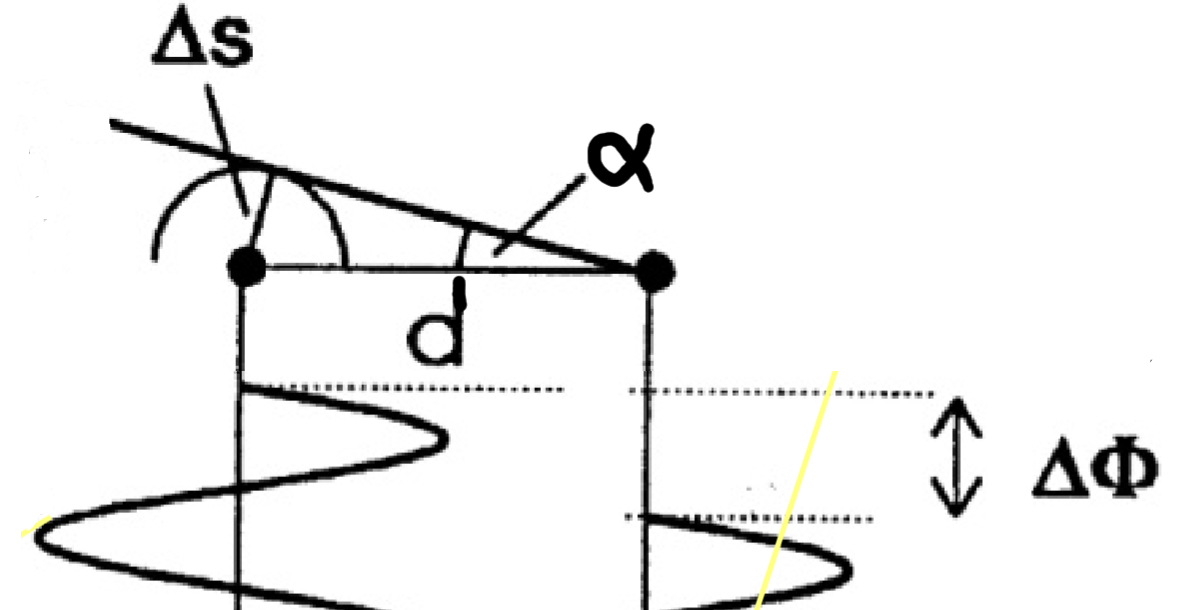
\includegraphics[width=\linewidth]{US_PhasedParallelMode}
\end{minipage}

Receiving analog: delay elements, then sum all up.

\textbf{Variable focusing} (with shifting) and a combination of all

\textbf{Multi-dim. arrays}: 2D or 1.5D ($1/2$ D = ``\textbf{elevation}'').

\textbf{Curved arrays} (instead of flat): For small acoustic windows

\textbf{Annular Array} (circular sections): Simpler adjustable focus and circular symmetry = more \textbf{isotropic depiction}
%%%%%%%%%%%%%%%%%%%%%%%%%%%%%%%%%%%%%%%%%%%%%%%%%%%%%%
\subsection{Scanning modes}
%
\textbf{A-Mode} (Amplitude): time (distance) vs amplitude. \\
Usage: e.g. measuring the thickness

\textbf{M-Mode} (Motion): time vs depth. Amplitude with brightness. Must be tilted manually

\textbf{B-Mode} (Brightness): 2D spacial. Amplitude with brightness

\textbf{Scanning Procedures}:\\
$\bullet$ \textbf{Parallel scan} for large acoustic window.
$\bullet$ \textbf{Sector scan} for small ac. window.
$\bullet$ \textbf{Radial scan} for transd. in blood vessels (measuring the vessel wall).
$\bullet$ \textbf{Compound scan} from different directions $\to$ redundancy and reduce speckles.
%%%%%%%%%%%%%%%%%%%%%%%%%%%%%%%%%%%%%%%%%%%%%%%%%%%%%%
\subsection{Measuring the blood flow}
%
Observer at velocity $v$, receives $f\ap{eff} = f \frac{c + v}{c}$

Blood vessel flows under the receiver with angle $\theta$ rel. to the vertical to transducer:
\fbox{$f\ped{rec} = f_i \frac{2 f_i \cos \theta}{c} + \frac{f_i v^2 \cos^2 \theta}{c^2}$}\\
\begin{minipage}{0.6\linewidth}
    \highlight{$\displaystyle f_D = f_i - f\ped{rec} \approx \frac{2 f_i v \cos \theta}{c}$}
\end{minipage}
\begin{minipage}{0.4\linewidth}
    Must know $\theta$ \\$\implies$ do B-Mode scan first
\end{minipage}

Red blood cells $\approx 7 \unit{\mu m}$ wide $\implies$ Use high freq., typ. 5MHz

\textbf{Cont. setup}: Separated receiver/transmitter. Quadr. encoder: Mult. with cos ($\to$ real part) and sin ($\to$ imag part) $\to$ double sided spectrum. Neg. side is \textit{negative flow}. Then \textit{low-pass + high-pass} to remove (quasi) stationary echos.

\textbf{Pulsed measurement}: 1 transducer. Only receive signal during a narrow time window. Its delay = depth.

\begin{minipage}{\linewidth}
    \raggedleft
    \vspace{2mm}
    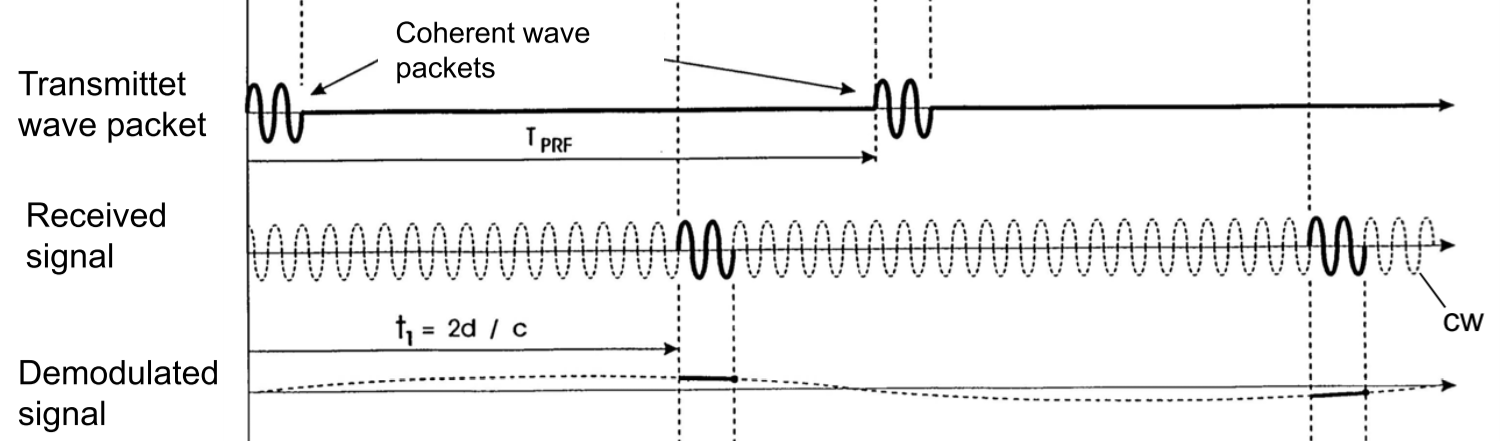
\includegraphics[width = \linewidth]{US_DopplerPulsed} \vspace{-37mm}\\
    \highlight{$\displaystyle -f\ped{prf}/2 < f\ped{D} < f\ped{prf}/2$}
    \vspace{37mm}
\end{minipage}
%%%%%%%%%%%%%%%%%%%%%%%%%%%%%%%%%%%%%%%%%%%%%%%%%%%%%%
\subsection{Appendix}
%
\begin{tabular}{ c@{$\;\laplace\;$}c c c@{$\;\laplace\;$}c }
    $f(at)$			& $\frac{1}{\abs{a}}F(s/a)$	&& $f(t-a)$		& $\eu^{-as}F(s)$\\
    $f(t)\eu^{at}$	& $F(s-a)$					&& $f'(t)$		& $sF(s) - f(0^+)$\\
    $t^n$			& $n!/s^{n+1}$				&& $t^n f(t)$	& $(-1)^n F^{(n)}(s)$\\
    $\sin(at)$		& $\frac{a}{s^2 + a^2}$		&& $\cos(at)$	& $\frac{s}{s^2 + a^2}$\\
    $\eu^{at}$		& $\frac{1}{s - a}$			&& $t^n \eu^{at}$& $\frac{n!}{(s-a)^{n+1}}$
\end{tabular}

\textbf{Constants}:\\
\begin{tabular}{r@{$\;=\;$}l}
    $h$			& $\unit[6.626\E{-34}]{JS} = \unit[4.135\E{-15}]{eV\,s}$,\qquad $\hbar = \frac{h}{2\pi}$\\
    $\epsilon_0$& $\unitfrac[8.85\E{-5}]{As}{Vm}$\\
    $\mu_0$		& $\unitfrac[4\pi\E{-7}]{N}{A^2}$\\
    $k\ped{B}$	& $\unitfrac[1.38\E{-23}]{J}{K} = \unitfrac[8.617\E{-5}]{eV}{K}$\\
    $q$			& $\unit[1.602\E{-19}]{C}$, \quad $m_e = \unit[9.109\E{-31}]{kg}$, \quad $m_p = \unit[1.672\E{-27}]{kg}$\\
    $m_ec^2$	& $\unit[511]{eV}$
\end{tabular}
$\unit[0]{^\circ C} = \unit[273.15]{K}$
